\documentclass[12pt]{article}
\usepackage[a4paper, total={7in, 10in}]{geometry}
\usepackage{multicol}
\usepackage{float}
\usepackage{tikz}

\begin{document}
\begin{Huge}

\begin{center}
•\textbf{ELEN3016: CONTROL LAB 1}\\
\end{center}
\end{Huge}\textbf{Group 7}\\\texttt{Tyson Cross (1239448)\\
Jannes Smit (10382530\\
Daniel de Barros (1036613)\\
}\section{Question 1}
\subsection{Matlab Simulations}
\begin{multicols}{2}
\begin{flushleft}
\begin{figure}[H]
\centering
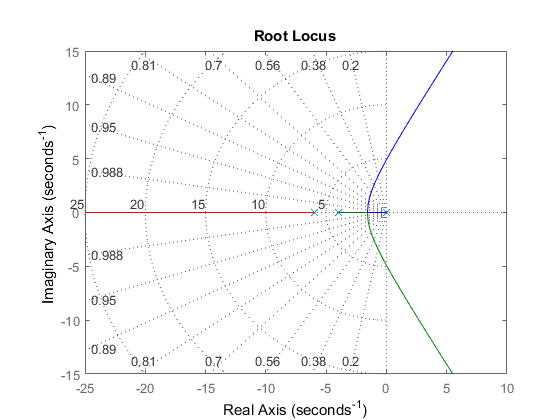
\includegraphics[scale=0.7]{Plant_Root_Locus.png}
\caption{Root-Locus Plot of Plant Transfer Function}
\end{figure}

\begin{figure}[H]
\centering
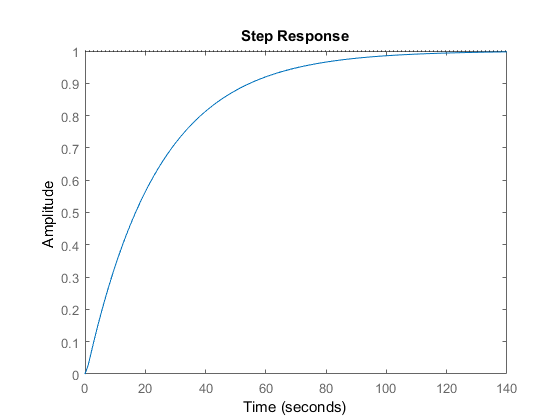
\includegraphics[scale=0.7]{StepResponse.png}
\caption{Step Response of Plant with Unity Feedback}
\end{figure}
\end{flushleft}
\end{multicols}

\begin{figure}[H]
\centering
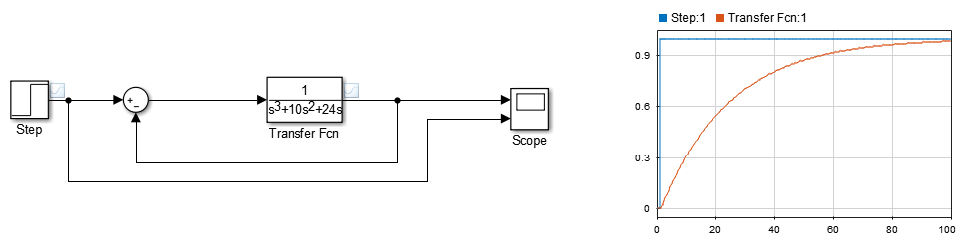
\includegraphics[scale=0.75]{Simulink.png}
\caption{Simulink Simulation}
\end{figure}

\begin{figure}[H]
\centering
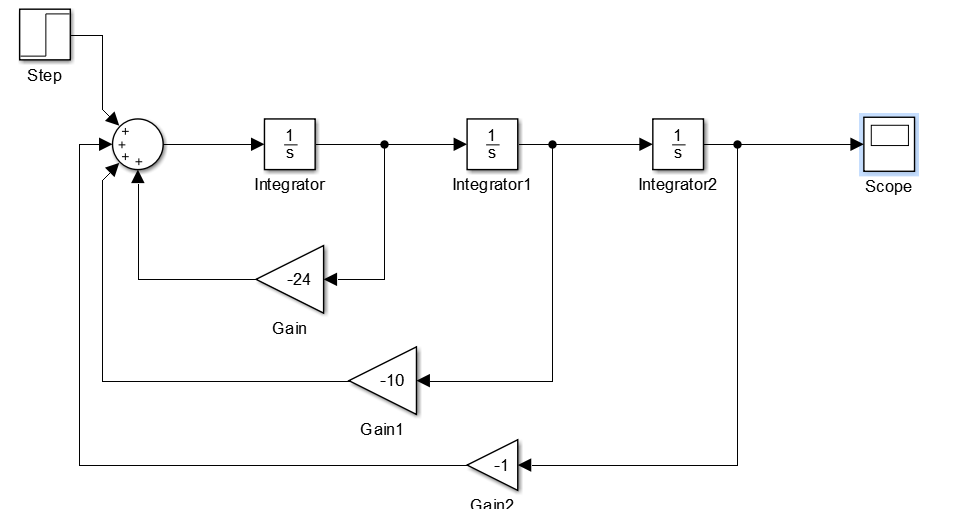
\includegraphics[scale=0.7]{State_Diagram.png}
\caption{Simulink Simulation}
\end{figure}
\end{document}